\begin{frame}
    \begin{center}
        \vspace{3.0cm}
        \normalsize
        \textbf{Игровые программы. Основы проектирования.} \\
        \vspace{1.5cm}
        \raggedleft\small\textbf{Выполнил:}\\Голубев~А.~В.\\САПР-1.1п\\
        \vspace{1.8cm}
        \vspace{\fill}
        \centeringВолгоград \the\year
    \end{center}
\end{frame}

% скрины
% \begin{figure}
%     \begin{minipage}{0.47\textwidth}
%         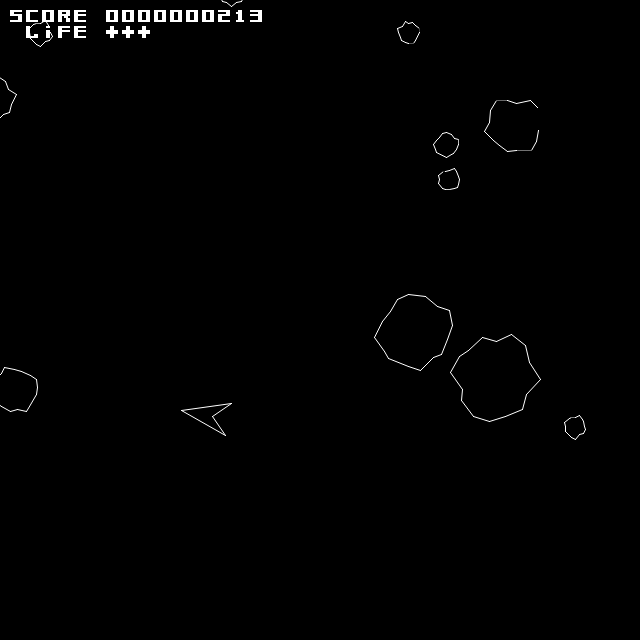
\includegraphics[width=1.0\textwidth]{scrshot01}
%     \end{minipage}
%     \begin{minipage}{0.47\textwidth}
%         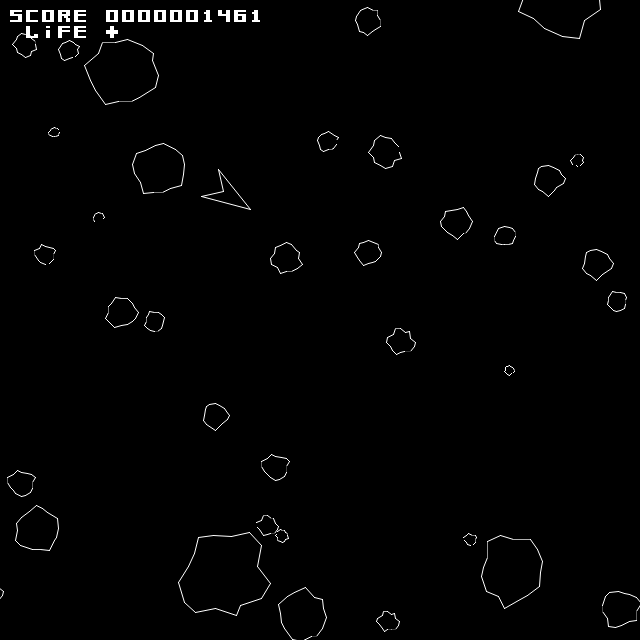
\includegraphics[width=1.0\textwidth]{scrshot02}
%     \end{minipage}
% \end{figure}

\begin{frame}
    \frametitle{Цели и задачи проекта}

    \emph{Целью создания} системы является:
    \begin{itemize}
        \item разработка электронного методического пособия по разработке структуры игровой программы
        \item создание игрового приложения базирующееся на данной структуре
    \end{itemize}

    Основным функциональным назначением системы является:
    \begin{itemize}
        \item представление базовой структуры в проектировании игровых программ
        \item ознакомление с основными алгоритмами используемыми в разработке
        \item предоставление студенту базовых знаний работы с SDL2, SDL2 image, 
            OpenAL, libvorbis
    \end{itemize}
\end{frame}

\begin{frame}
    \frametitle{Описание объекта автоматизации}
\end{frame}

\begin{frame}
    \frametitle{Функциональная структура АС}
    % добавить текст на слайд
    \begin{figure}
        \centering
        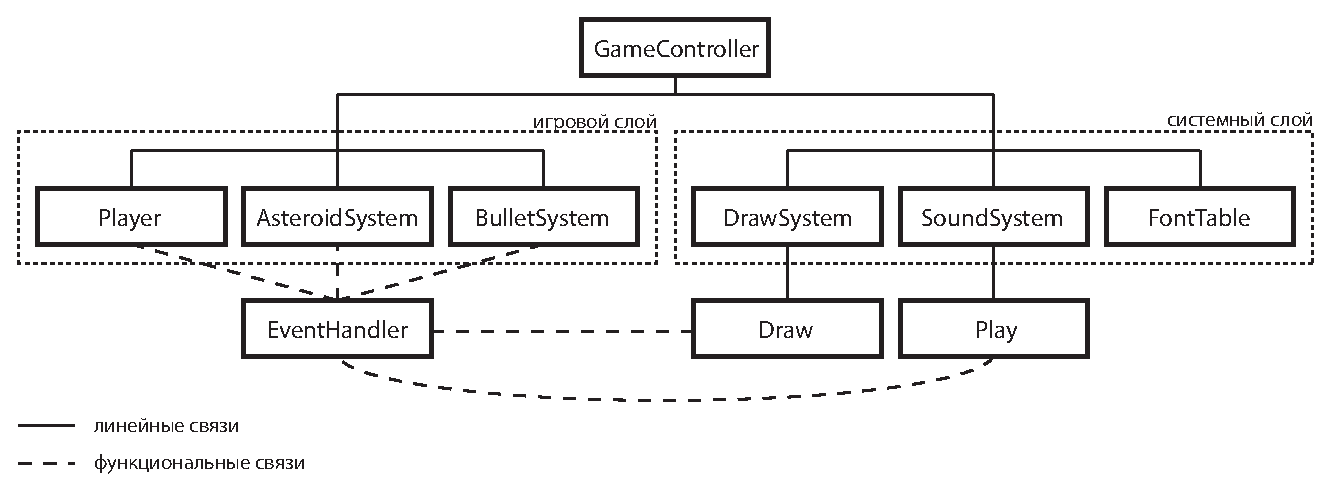
\includegraphics[width=1.0\textwidth]{functional_system}
    \end{figure}
\end{frame}

\begin{frame}
    \frametitle{Функциональная структура АС}
    % добавить текст на слайд
    \begin{figure}
        \centering
        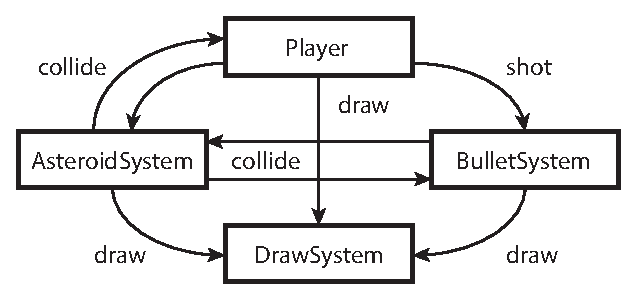
\includegraphics[width=1.0\textwidth]{system_handler}
    \end{figure}
\end{frame}

\begin{frame}
    \frametitle{Описание входных и выходных данных АС}

    \emph{Входные данные}:
    \begin{itemize}
        \item загружаемые ресурсы
        \item действия пользователя
    \end{itemize}
    \emph{Выходные данные}:
    \begin{itemize}
        \item реакция игровой логики
        \item графическая визуализация 
    \end{itemize}
\end{frame}

\begin{frame}
    \frametitle{Логическая структура АС}
    % добавить текст на слайд
    \begin{figure}
        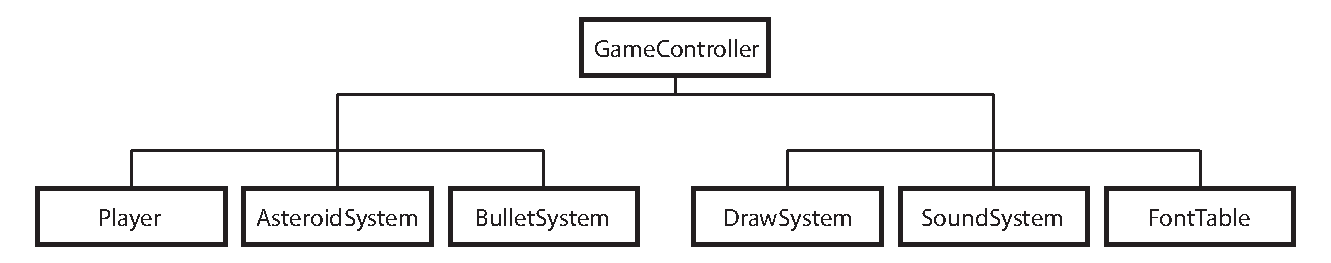
\includegraphics[width=1.0\textwidth]{logic_struct}
    \end{figure}
\end{frame}

\begin{frame}
    \frametitle{Архитектура АС}
    % \begin{figure}
    %     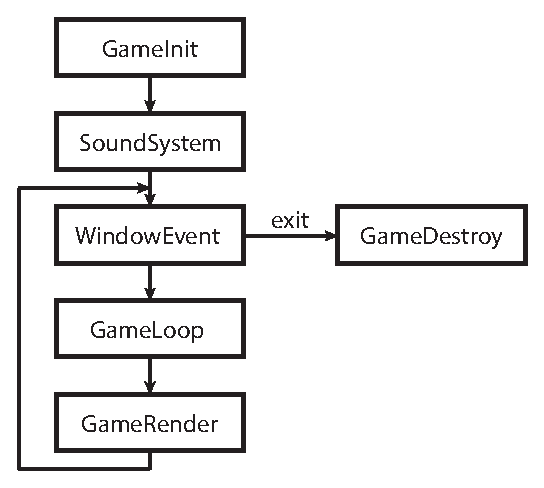
\includegraphics[width=0.6\textwidth]{game_system}
    % \end{figure}
\end{frame}

\begin{frame}
    \frametitle{Выводы}
\end{frame}